\documentclass[11pt]{book}
\usepackage[bottom=2cm,
  top=3cm, left=3cm, right=2cm]{geometry}
\usepackage[italian]{babel}
\usepackage{amsmath}
\usepackage{graphicx}
\usepackage{todonotes}

\setlength{\parindent}{0pt}

\begin{document}
\setcounter{chapter}{2}
\chapter{La gerarchia delle memorie}

Nelle prime CPU si utilizzava l'architettura di Von Neumann che
prevedeva tre blocchi (CPU, Memoria ed Interfacce) collegate da un
bus. Durante l'esecuzione di un programma la CPU alternava sempre
stati di fetch (IF) a stati di esecuzione (EX). Trascuriamo per il
momento le altre fasi. Ogni operazione richiedeva l'accesso in
memoria, dunque sebbene le unit\`a funzionali fossero molto veloci
(vedi la ADD) i tempi di esecuzione erano molto grandi dovendo
prelevare dalla memoria gli operandi e scriverci il risultato. Le
performance erano quindi fortemente influenzate da quelle della
memoria. L'architettura era molto sbilanciata.

\par\bigskip

Un'altra problematica delle vecchie CPU era che, se la memoria era di
64 KB, non potevano essere eseguiti programmi di dimensione
maggiore. Questo problema fu risolto grazie all'introduzione della
{\bf memoria virtuale}: ogni programma vedeva uno spazio di
indirizzamento di 4 GB, indipendentemente dalla memoria fisicamente
disponibile sul calcolatore. In realt\`a vi era un'altra soluzione,
gli overlay, ma non la trattiamo. Tornando alla memoria virtuale, il
software richiede l'accesso a indirizzi di memoria virtuale, da questi
si ricava il corrispondente indirizzo fisico se il dato in memoria
c'\`e, altrimenti l'hardware genera un {\bf page fault}. Se la pagina
non c'\`e \`e il sistema operativo che prende la pagina e la porta in
memoria fisica. La memoria virtuale consente dunque di svincolare il
programmatore ed il programma dalla dimensione della memoria fisica
tramite un meccanismo misto hardware/software. L'hardware deve
rilevare il page fault, il software deve portare il dato in memoria
fisica.

\par\bigskip

Il primo problema viene invece risolto utilizzando un altro livello di
memoria interna alla CPU. Non pu\`o essere grande quanto lo spazio
virtuale, ma \`e molto limitata. La condizione ideale sarebbe avere
tempo di accesso in memoria pari al tempo di accesso in cache, cio\`e
un clock, e dimensione del programma pari alla dimensione della
memoria virtuale. Per avere ci\`o bisogna dimensionare adeguatamente i
parametri dell'architettura della memoria e facendo in modo che siano
rispettati quanto pi\`u possibile i principi di localit\`a spaziale e
temporale.

\par\bigskip

Si introducono perci\`o tre livelli di memoria organizzati
gerarchicamente. Il livello pi\`u elevato \`e la {\bf cache}, seguono
la {\bf memoria centrale} e la {\bf memoria virtuale}. Per riuscire a
implementare dei meccanismi di controllo degli accessi alla memoria
\`e stata introdotta anche la {\bf memoria segmentata} (che \`e il
livello pi\`u basso).

\begin{figure}[h]
  \centering
  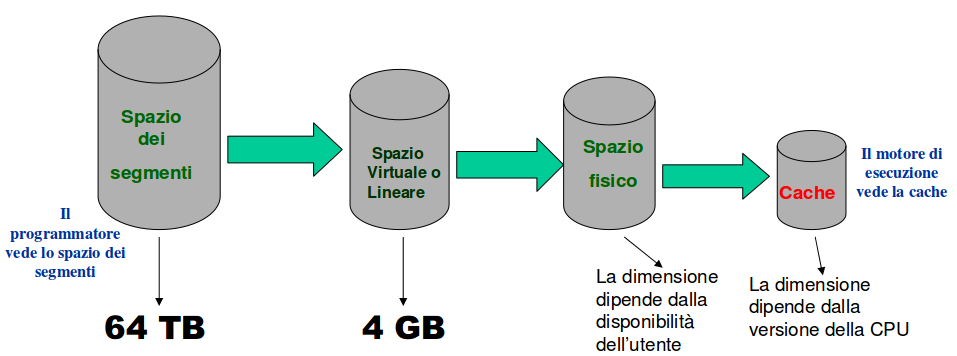
\includegraphics[width=.9\textwidth]{images/gerarchia.png}
  \caption{Gerarchia della memoria}
  \label{gerarchia}
\end{figure}

\section{La catena di traduzione degli indirizzi}

Supponiamo di voler fare {\tt MOV AL PIPPO}. Il funzionamento della
gerarchia \`e il seguente: la CPU cerca il dato nel livello pi\`u
vicino (cache). Se c'\`e, dunque ho una {\bf Hit} in cache, vi si accede in
un clock. Devo per\`o avere l'indirizzo del dato cercato in
cache. Come lo ottengo? Tramite la catena di traduzione degli
indirizzi. {\tt PIPPO} \`e un nome simbolico che il compilatore
tradurr\`a in un numero: questo \`e l'indirizzo nello spazio dei
segmenti. Si tratta perci\`o della combinazione Segmento +
Offset. Questo \`e il primo livello di traduzione. Attraverso il
descrittore del segmento situato in LDT riusciamo a tradurre in
indirizzo virtuale. Da questo, tramite ad esempio la {\em directory},
traduco in indirizzo fisico e dall'indirizzo fisico ho direttamente
l'indirizzo in cache (vedere la sezione relativa alla cache). 

\par\bigskip

Se invece ho una {\bf Miss} in cache, vado al livello successivo,
cio\`e la memoria centrale. Se l'informazione cercata \`e presente in
memoria centrale la copio in cache (copio l'intero blocco la cui
dimensione varia a seconda della dimensione delle linee di cache) e
quindi ri-accedendo alla cache avr\`o finalmente la Hit. Se non \`e
presente nemmeno in memoria centrale, la cerco nel livello successivo,
cio\`e la memoria virtuale. In questo caso prendo una pagina di 4 KB e
la porto in memoria centrale. Posso perci\`o ritornare in memoria
centrale dove questa volta il dato verr\`a trovato e successivamente
portato in cache. La probabilit\`a di Miss \`e bassa dato che si cerca
di rispettare il principio di localit\`a spaziale e temporale,
perci\`o questo processo oneroso verr\`a svolto poche volte. Il {\bf
  principio di localit\`a spaziale} afferma che i dati spazialmente
vicini a quelli appena acceduti hanno maggiori probabilit\`a di essere
richiesti; viene rispettato portando in cache dei blocchi di grandi
dimensioni contenenti il dato richiesto (anzich\'e portare soltanto il
dato). Il {\bf principio di localit\`a temporale} invece, afferma che
un dato utilizzato recentemente con molta probabilit\`a verr\`a
riutilizzato; tale principio viene rispettato sostituendo in cache le
informazioni accedute meno recentemente.

\par\bigskip

A ogni livello e a ogni blocco deve essere associato un
descrittore. Il descrittore dice se il blocco cercato \`e presente o
meno nel livello adiacente settando il {\bf bit present}
rispettivamente a 1 o a 0. Nel primo caso, il descrittore conterr\`a
anche l'indirizzo del blocco nel livello adiacente. In caso contrario
deve dare le informazioni necessarie a reperirlo per portarlo nel
livello adiacente.

\section{Il livello pi\`u basso: la Memoria logica}

\subsection{Funzionamento di base}

Lo \textbf{spazio dei segmenti} \`e ci\`o che vede il
programmatore. Ogni task pu\`o avere associati uno o pi\`u {\bf
  segmenti} di memoria (ad esempio segmento dati, segmento codice,
ecc\dots). Ogni segmento pu\`o avere dimensione massima di 4 GB e ha
associato un {\bf descrittore}. Prima di analizzare nel dettaglio le
strutture coinvolte, diamo una panoramica del funzionamento della
memoria logica.

\

Il {\bf descrittore del segmento} ha dimensione di 8 byte e contiene
tutte le caratteristiche del segmento stesso. I descrittori sono
riuniti in due {\bf tabelle dei descrittori}. Una \`e {\bf globale}
(\textbf{GDT}) ed accessibile tramite il registro \texttt{GDTR},
l'altra \`e locale ed accessibile tramite il registro
\texttt{LDTR}. Ogni task vede la tabella globale ed una sua tabella
locale. Ogni tabella contiene 8 K descrittori, pertanto la dimensione
di ognuna di queste tabelle \`e di 8 byte $\cdot$ 8 K descrittori = 64
K. Dal momento che di tabelle ogni task ne vede due, avr\`a a
disposizione 16 K descrittori; ogni descrittore fa riferimento ad un
segmento che \`e grande fino a 4 GB, perci\`o l'area di memoria
visibile ad ogni task \`e di 4 GB $\cdot$ 16 K = 64 TB.

\

Ai descrittori si accede tramite un {\bf selettore} da 16 bit che
contiene sia le informazioni riguardanti la tabella di appartenenza
(LDT o GDT), sia l'indice del descrittore nella tabella.

Ricapitolando:
\begin{itemize}
\item dimensione massima di un segmento: 4 GB
\item dimensione di un descrittore: 8 byte
\item numero di descrittori per tabella: 8 K
\item dimensione di una tabella: 8 byte $\cdot$ 8 K = 64 K
\item numero di descrittori visibili ad un task: 16 K
\item dimensione della memoria visibile ad un task: 4 GB $\cdot$ 16 K
  = 64 TB
\end{itemize}

64 Terabyte \`e un numero {\em commerciale} perch\'e i segmenti sono
tutti pi\`u piccoli di 4 GB ed inoltre le tabelle dei descrittori non
contengono soltanto descrittori dati, stack e codice, ma anche
descrittori di altri oggetti visibili alla CPU, ad esempio i
descrittori dei task. Quindi lo spazio che ogni task vede non sar\`a
mai di 64 Tera, ma sicuramente inferiore.

\subsection{Struttura del selettore}

Il selettore, come detto, \`e di 16 bit organizzati come segue:

\begin{center}
\begin{tabular}{|c|c|c|}
\hline
13 bit di indice & 1 bit T1 & 2 bit RPL \\
\hline
\end{tabular}
\end{center}

\begin{itemize}
\item i 13 bit di indice permettono di indirizzare $2^{13} = 8 K$
  locazioni, quindi ogni posizione di una delle due tabelle;
\item il bit \texttt{T1} vale 1 se l'indirizzo specificato nel campo
  precedente \`e della LDT, 0 se della GDT;
\item gli ultimi due bit son detti \texttt{RPL}, {\em Requestor
    Privilege Level} e servono a indicare il livello di privilegio del
  segmento di codice che ha generato il selettore.
\end{itemize}

\subsection{Struttura del descrittore}

La struttura generica di un descrittore \`e la seguente:

\begin{figure}[h]
  \centering
  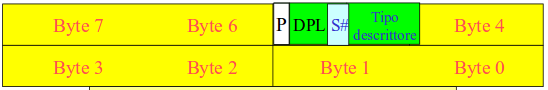
\includegraphics[width=.6\textwidth]{images/descrittore.png}
  \caption{Struttura generica di un descrittore}
  \label{descrittore}
\end{figure}

Il {\bf tipo di descrittore} \`e il campo che ci consente di
discriminare tra descrittori di segmento dati, codice, di task o di
altri oggetti. Vediamo la struttura dei descrittori di segmento dati e
di quelli di codice.

\subsubsection{La struttura del descrittore di un segmento dati}

Il {\bf descrittore di segmento dati} \`e rappresentato in figura
\ref{descrittoredati} e contiene i seguenti campi:

\begin{figure}[h]
  \centering
  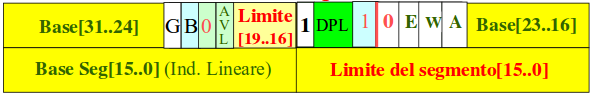
\includegraphics[width=.6\textwidth]{images/descrittoredati.png}
  \caption{Struttura di un descrittore di segmento dati}
  \label{descrittoredati}
\end{figure}

\begin{itemize}
\item {\bf base}: \`e l'indirizzo iniziale del segmento \textbf{nella
    memoria virtuale} ed \`e composto dai 32 bit spezzettati in {\tt
    Base[31..24]}, {\tt Base[23..16]}, {\tt Base[15..0]}
\item {\bf limite del segmento}: \`e l'offset massimo a cui possiamo
  andare in quel segmento. \`E composto da 20 bit ({\tt
    Limite[19..16]} e {\tt Limite[15..0]}) quindi potrei avere
  soltanto 1 MB come lunghezza massima dei segmenti. Cosa succede se
  il segmento \`e pi\`u lungo di 1 MB? Possiamo dunque utilizzare
  un'altra unit\`a di misura invece del byte: le pagine di 4 KB. In
  questo modo possiamo arrivare ad avere segmenti di 4 GB (perch\'e $4
  KB = 2^2 \cdot 2^{10}$ e questo valore va moltiplicato per 1 MB che
  \`e $2^{20}$). Per sapere se si stanno usando i byte o le pagine di
  4 KB si utilizza il campo contrassegnato da {\bf G}. Se vale 0 si ha
  granularit\`a 1 byte, altrimenti 4 KB. Questo limite ci permette di
  fare un controllo fondamentale che ci consente di non sforare,
  quindi di non accedere a segmenti di altri task. Si fa in modo da
  accedere sempre all'interno del proprio segmento

\item {\bf due altri byte} (precisamente il 5 e il 6) in cui sono
  immagazzinate alcune informazioni fra cui:

  \begin{itemize}
  \item {\bf G}: lo abbiamo gi\`a visto prima;
  \item {\bf Limite[19..16]}: gi\`a visto prima;
  \item {\bf P}: \`e il famoso bit {\bf present} ed indica se il
    segmento \`e mappato nel livello adiacente della gerarchia di
    memoria (cio\`e in questo caso in memoria virtuale);
  \item {\bf DPL}: \`e un campo di 2 bit e serve a controllare chi
    accede e a quale oggetto per verificare che l'accesso sia
    lecito. La sigla DPL sta per {\em Descript Privilege Level}. Se
    l'accesso non \`e lecito si genera un'eccezione che verr\`a poi
    gestita dal software;
  \item {\bf i due bit a fianco a DPL}: in questo caso valgono 10 ed
    individuano un descrittore di segmento dati. In generale il bit
    pi\`u significativo in questa coppia \`e chiamato {\bf S\#} e se
    vale 0 indica un descrittore di un {\em oggetto di sistema},
    mentre se vale 1 indica un descrittore di tipo dati (come in
    questo caso) o codice. {\bf S} sta per System;
  \item {\bf W}: \`e un bit appartenente al campo che indica il tipo di
    descrittore e vale 1 se il segmento \`e anche scrivibile, 0 se lo si
    pu\`o solo leggere.
  \item {\bf A}: sta per {\em Accessed} e viene settato a 1
    automaticamente ogni volta che si fa l'accesso al
    segmento. Sappiamo che ogni segmento viene mappato in memoria
    virtuale quando deve essere utilizzato; se la memoria virtuale \`e
    piena bisogna decidere quale segmento gi\`a mappato in memoria
    virtuale dobbiamo sostituire. Per fare ci\`o si sceglie
    solitamente quello acceduto meno di recente sfruttando l'algortimo
    {\em LRU} o, in maniera meno onerosa, con un algoritmo
    pseudo-LRU. Il bit A viene azzerato ogni $\delta T$ per tutti i
    segmenti. In un intervallo fra un reset e l'altro alcuni segmenti
    potrebbero essere utilizzati e dunque avere nuovamente
    $A=1$. Quelli che restano con $A=0$ sono dunque i segmenti
    utilizzati meno recentemente e perci\`o gli unici candidati alla
    sostituzione.
\end{itemize}
\end{itemize}

\subsubsection{La struttura del descrittore di un segmento codice}

\begin{figure}[h]
  \centering
  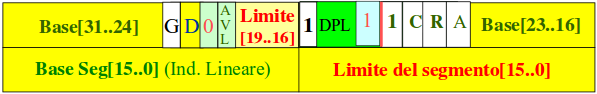
\includegraphics[width=.6\textwidth]{images/descrittorecodice.png}
  \caption{Descrittore del segmento codice}
  \label{descrittore codice}
\end{figure}

Molti dei campi che lo compongono li abbiamo gi\`a visti. Gli altri
sono:

\begin{itemize}
\item Il {\bf bit D} serve a determinare il linguaggio macchina (ISA)
  che stiamo utilizzando. Con $D=0$ utilizzo un determinato ISA, con
  $D=1$ ne uso uno differente. Questo \`e stato necessario perch\'e al
  momento dell'introduzione dell'architettura a 32 bit i sistemi
  operativi disponibili erano per lo pi\`u a 16 bit. Tramite questo
  campo si effettuava quindi un downgrade della CPU per farla
  funzionare a 16 bit. Se invece di un bit ne avessimo due, potremmo
  addirittura pensare di far supportare alla nostra macchina anche il
  codice ARM (ad esempio).

\item Il {\bf bit R} vale 0 se il segmento di codice pu\`o essere
  usato solo dalla CPU in fase di fetch per l'esecuzione, cio\`e
  contiene solo istruzioni; vale 1 quando lo posso anche leggere, non
  solo eseguire. Ci\`o \`e possibile quando si tratta di un segmento
  che si trova in EPROM e che quindi essendo non volatile mi permette
  anche di memorizzarci delle costanti.
\end{itemize}

Per capire che si tratta di un segmento codice si osservano i due bit
situati dopo il DPL che in questo caso sono posti a 11.

\subsection{I livelli di privilegio}

Vediamo dunque quali sono i {\bf livelli di privilegio}. Ogni
programma quand'\`e in esecuzione gira ad un determinato livello di
privilegio. Le applicazioni semplici sono poco privilegiate, mentre il
sistema operativo ha il livello di privilegio massimo (anche se pu\`o
differire a seconda dei suoi componenti). I livelli sono 4 e vanno
dallo 0 (il pi\`u privilegiato) a 3 (il meno privilegiato). In un
segmento il livello di privilegio \`e indicato dai due bit {\bf DPL}
(infatti 2 bit possono indicare al massimo 4 livelli), mentre l'{\bf
  RPL} contiene il livello di privilegio di chi genera un selettore
per accedere ad un segmento.

Tramite il PC (Program Counter) posso sapere quale segmento di codice
\`e in esecuzione perch\'e fornisce delle coppie (CS, IP), cio\`e il
Code Segment e l'Instrucion Pointer. Mentre l'IP indica l'offset nel
segmento di codice attivo, il {\bf Code Segment} \`e un registro che
contiene proprio questo segmento codice ed il suo selettore. Gli
ultimi due bit del selettore presente nel CS, dato che \`e il segmento
attivo in quel momento, li chiamiamo {\bf CPL} ovvero {\em Current
  Privilege Level}. Questo sar\`a in generale uguale al DPL del
segmento di codice che contiene quell'istruzione.

La CPU utilizza i livelli di privilegio per fare il controllo degli
accessi. Il controllo degli accessi viene fatto quando il codice
richiama altro codice (cio\`e chiamiamo ad esempio una procedura e
dobbiamo fare il trasferimento del controllo) oppure quando il codice
accede ai dati (con delle load o store). Ogni segmento ha il suo CPL,
quindi si segue questa regola: 

\begin{itemize}
\item posso solo chiamare codice con livello di privilegio uguale o
  superiore;
\item  posso leggere solo dati con livello di privilegio uguale o
  inferiore.
\end{itemize}

Quindi il controllo da fare, nel momento in cui si accede a dei dati,
\`e che il CPL sia minore o uguale del DPL del segmento dati (e quindi
che il codice sia pi\`u privilegiato).

\par\bigskip

\underline{{\bf TODO}: call gate}

\section{Da Memoria Logica a Memoria Virtuale}

\subsection{La Memoria virtuale}

La memoria virtuale \`e posta fra lo spazio dei segmenti e la memoria
fisica per evitare che i segmenti vengano mappati direttamente in
memoria fisica e lasciare quindi ad ogni software uno spazio di 4 GB
indipendente dalla dimensione della memoria fisica. La memoria
virtuale \`e nata quindi con lo scopo di ottimizzare l'uso della
memoria fisica.

\subsection{Indirizzi}

La memoria virtuale \`e di 4 GB, divisa in pagine di 4 KB. Un semplice
calcolo ci dice che all'interno di questa memoria abbiamo quindi:

$$
\frac{4 \text{ GB}}{4 \text{ KB}} = \frac{2^{32}}{2^{12}} = 2^{20}
\text{ pagine} = 1 M \text{ pagine}
$$

Per indirizzare ogni pagina avremo quindi bisogno di 20 bit (5 cifre
esadecimali). Dal momento che ogni pagina \`e da 4 KB, per indirizzare
un byte all'interno della pagina abbiamo bisogno di 12 bit (3 cifre
esadecimali). Ecco dunque che l'inirizzo virtuale si ottiene
affiancando ai 20 bit che selezionano la pagina (che chiamiamo
\texttt{IV[31..12]}) i 12 bit che indicano l'offset nella stessa
(\texttt{IV[11..0]}).

\

L'indirizzo di memoria virtuale si ottiene prendendo la \textbf{base}
contenuta nel descrittore di segmento (32 bit) e sommando ad essa
l'\textbf{offset} contenuto nel registro \texttt{EA}.

\section{Da Memoria virtuale a Memoria fisica}

\subsection{Indirizzi di memoria fisica}

Come nella memoria virtuale, la memoria fisica \`e organizzata in
pagine da 4 KB, dunque se una pagina di memoria virtuale viene copiata
in memoria fisica, l'offset rimane invariato. Fra indirizzo virtuale
ed indirizzo fisico rimarranno perci\`o identici i 12 bit meno
significativi (3 cifre esadecimali) e cambier\`a il \textbf{Page\_ID},
ancora i 20 bit. Una tabella, detta \textbf{Page Directory}, mantiene
la corrispondenza fra pagine di memoria virtuale e fisica. Svolge
quindi il ruolo di \textbf{Page Mapper}.

\subsection{La Page Directory (PD)}

La \textbf{Page Directory} \`e una struttura dati (residente in
memoria e puntata dal registro \texttt{CR3} della CPU) che ci permette
di ricavare l'indirizzo di una pagina di memoria fisica a partire da
quello di una pagina di memoria virtuale. Per ogni riga di memoria
virtuale abbiamo una riga in PD che contiene il Page\_ID fisico (se
tale pagina esiste in memoria fisica) ed il bit Present (che vale 1 se
la pagina esiste in memoria fisica, 0 altrimenti). L'indirizzo fisico
viene quindi ottenuto concatenando il Page\_ID fisico all'offset
costituito dalle 12 cifre meno significative dell'IV (indirizzo
virtuale). La PD contiene 1 M locazioni (perch\'e tante sono le
pagine) da 20 bit (perch\'e solo 20 servono ad individuare il
corrispondente indirizzo fisico). Questo schema \`e noto come
\textbf{mapping ad un livello} in quanto si attraversa solo la PD per
arrivare all'indirizzo fisico.

\

Uno schema alternativo \`e il \textbf{mapping a due livelli}. Qui
l'indirizzo virtuale \`e diviso in tre parti, non due come abbiamo
detto finora. Le tre parti sono:

\begin{itemize}
\item \texttt{IV[31..22]}: si indica con \textbf{PDE\_ID}.
\item \texttt{IV[21..12]}: si indica con \textbf{PTE\_ID}.
\item \texttt{IV[11..0]}: come detto \`e l'offset nella pagina.
\end{itemize}

A cosa serve questa suddivisione? Cos\`i facendo si ottiene una PD
pi\`u piccola, infatti avendo soltanto 10 bit di \texttt{PDE\_ID} si
hanno $2^{10}$ (cio\`e 1 K) locazioni (dette appunto \texttt{Page
  Directory Entry}). Ogni locazione punta ad una fra le $2^{10}$
possibili \textbf{Page Table}. Ognuna di queste contiene $2^{10}$
locazioni (dette \texttt{Page Table Entry}) visto che 10 sono anche i
bit del \texttt{PTE\_ID} e tramite queste tabelle si arriva a
selezionare una pagina. Questo schema \`e detto \textbf{Mapping a due
  livelli} perch\'e per arrivare ad ottenere l'indirizzo fisico da
quello virtuale si devono attraversare la Page Directory ed una Page
Table. Con questo metodo, la struttura residente in memoria (la PD)
\`e pi\`u piccola e le PT sono in memoria di massa e vengono caricate
in memoria centrale solo all'occorrenza. Lo svantaggio \`e che per\`o
ogni traduzione richiede due accessi in memoria.

\

Vediamo qual \`e la struttura delle \textbf{Page Directory} e delle
\textbf{Page Table}. Ogni riga in queste tabelle non contiene soltanto
l'indirizzo della pagina di memoria fisica, ma anche altre
informazioni. Tutte insieme compongono il \textbf{descrittore} che
possiamo vedere in figura \ref{pdpt}.

\begin{figure}[h]
  \centering
  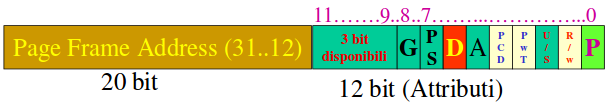
\includegraphics[width=.7\textwidth]{images/pdpt.png}
  \caption{Struttura di un descrittore della Page Directory}
  \label{pdpt}
\end{figure}

I campi che lo compongono sono:

\begin{itemize}
\item \texttt{P}: \`e il \textbf{bit Present} che indica se la
  relativa pagina virtuale \`e presente in memoria fisica;
\item \texttt{R/W}: se vale 1 indica che la scrittura \`e abilitata,
  altrimenti la pagina \`e protetta;
\item \texttt{U/S}: autorizzazione all'accesso (\textit{User} o
  \textit{Super User});
\item \texttt{PWT}: indica la \textbf{politica di scrittura in
    cache}; %% TODO: cioe?
\item \texttt{PCD}: sta per \textbf{cache disable} e si utilizza per
  disabilitare la scrittura in cache di tale linea;
\item \texttt{A}: sta per \textbf{accessed} e viene settato ad 1 ad
  ogni accesso alla pagina e rimesso a 0 allo scadere di un
  timer. Tale bit viene utilizzato per determinare quanto
  frequentemente si \`e acceduto a tale pagina;
\item \texttt{D}: sta per \textbf{dirty} e viene settato a 1 ogni
  volta che si modifica la pagina in memoria fisica. Ci\`o impedisce
  che tale pagina venga sovrascritta prima di essere copiata in
  memoria virtuale;
\item \texttt{PS}: sta per \textbf{page size} e si utilizza perch\'e
  in determinati sistemi si possono avere, oltre alle classiche pagine
  da 4 KB, anche pagine da 4 MB, particolarmente utili quando si
  maneggiano grossi file;
\item \texttt{G}: \textbf{global}, indica che una pagina in memoria
  \`e globale, per cui non viene invalidata nel \texttt{TLB} quando si
  aggiorna \texttt{CR3} o quando c'\`e una commutazione di task.
\end{itemize}

La Page Directory e le Page Table sono mappate in memoria fisica
quando la CPU deve tradurre un indirizzo virtuale in indirizzo fisico,
mentre sono mappate in memoria virtuale quando devono essere
aggiornate dal gestore della memoria (che \`e un componente del
sistema operativo e in quanto tale vede solo la memoria virtuale). Per
questo motivo, per evitare incongruenze, la PD e le PT sono mappate
con gli stessi indirizzi sia nello spazio virtuale che in quello
fisico. Questo \`e quello che si chiama \textbf{Mapping Identico}.

\

Dal momento che ogni task vede le sue pagine di memoria virtuale, ogni
qual volta si cambi task si cambia la Page Directory e di conseguenza
l'indirizzo contenuto in \texttt{CR3}.

\subsection{TODO -- Le pagine da 4 MB}

%% TODO: le pagine da 4 MB

\subsection{Accelerare la traduzione da IV a IF}

Possiamo definire il \textbf{working set} di un programma come
l'insieme degli indirizzi a cui tender\`a ad accedere pi\`u
spesso. L'indirizzo base di queste pagine viene quindi mantenuto in
una memoria associativa (vedi sezione \ref{chap:memorieassociative}),
la \textbf{TLB} (\textit{Translation Look-aside Buffer}) allo scopo di
velocizzare l'accesso. Essendo una memoria associativa \`e organizzata
in coppie Nome-Valore. Qui il nome \`e dato dai bit
\texttt{IV[31..12]}, mentre il valore da
\texttt{IF[31..12]}. Solitamente i TLB sono memorie set-associative.

\

Nel momento in cui si cambia task, dato che cambia la Page Directory
(e che cambiano anche le pagine a cui accede pi\`u frequentemente il
task) si deve fare il \textbf{flush} del \texttt{TLB}. Per preservare
delle entry nella \texttt{TLB} si pu\`o settare il bit \texttt{G} del
relativo descrittore. Tale bit rende infatti globale la relativa
pagina e se ne evita la cancellazione dal \texttt{TLB}.

\ 

Relativamente al \texttt{TLB} c'\`e da dire che il Pentium dispone di
3 \texttt{TLB}:

\begin{itemize}
\item uno per le pagine di codice con 32 elementi ()
\item uno per le pagine di dati da 4 KB con 64 elementi
\item uno per le pagine di dati da 4 MB con 8 elementi
\end{itemize}

\subsection{Riepilogo}

La traduzione da indirizzo virtuale a indirizzo fisico pu\`o quindi
essere svolta come in figura \ref{ivif}.

\begin{figure}[h]
  \centering
  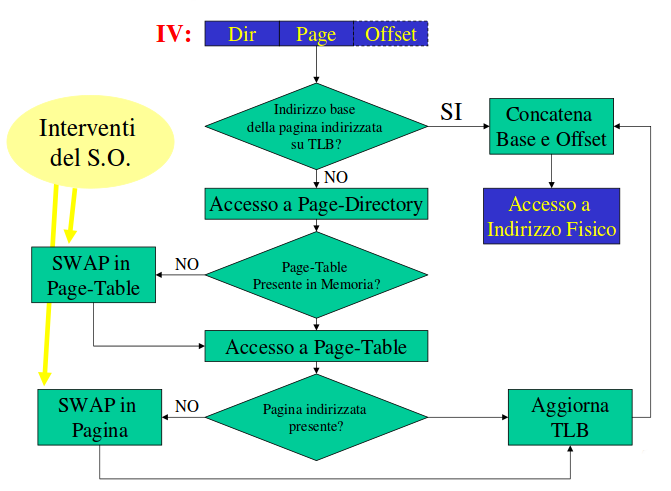
\includegraphics[width=.9\textwidth]{images/ivif.png}
  \caption{Traduzione da IV a IF}
  \label{ivif}
\end{figure}

\section{Da Memoria Fisica a Cache}

\subsection{La Cache}

La {\bf cache} \`e una {\bf memoria associativa} (vedi Appendice
\ref{chap:memorieassociative}), cio\`e una {\bf CAM} ({\em Content
  Access Memory}). Avendo un indirizzo fisico, si accede alla cache e
si recupera la relativa linea di cache. La cache \`e organizzata in
linee di 32 byte, quindi all'interno di ogni linea, ogni byte \`e
indirizzabile con $5$ bit di {\bf offset}. Le informazioni contenute
nella cache provengono dalla memoria fisica: il trasferimento avviene
tramite i {\bf cicli burst} che trasferiscono 32 byte per volta.

\subsection{Gli indirizzi}

L'indirizzo di una linea di cache pu\`o essere facilmente ricavato a
partire dall'indirizzo fisico con il quale c'\`e una
corrispondenza. Sappiamo intanto che le linee di cache sono di 32
byte, quindi per indirizzare un byte all'interno di una linea di cache
abbiamo bisogno di 5 bit. Possiamo pertanto dire che i 5 bit meno
significativi dell'indirizzo fisico vanno a costituire
l'\textbf{offset} nella linea.

Cosa ne facciamo degli altri 27 bit? Ci\`o dipende dal tipo di cache
che stiamo adottando. Vediamo dunque nello specifico i tre possibili
casi (ricordiamo che i vari tipi di cache sono descritti in
\ref{chap:memorieassociative}):

\begin{itemize}
\item \textbf{Cache Fully Associative}: ricordiamo prima di tutto che
  in queste cache i 32 byte di memoria fisica che vogliamo memorizzare
  in cache possono essere memorizzati in una qualunque
  posizione. Nelle cache fully associative abbiamo un solo set e tante
  vie (dunque altrettanti comparatori). Non avremo pertanto la
  necessit\`a di selezionare un set, quindi tutti i 27 bit verranno
  usati come \textbf{Line\_ID}. Si inviano questi 27 bit a tanti
  comparatori quante sono le vie e si effettua in ogni comparatore il
  confronto fra quei 27 bit ed il tag memorizzato nella relativa via
  per vedere se la riga \`e quella cercata.

\item \textbf{Cache Set Associative}: queste cache sono una via di
  mezzo fra le fully associative e quelle a mapping diretto, nel senso
  che per ogni set si comportano come cache fully
  associative. Possiamo ottenere una cache set associative partendo da
  una a mapping diretto e dividendola in due. Otteniamo una cache a
  due vie. Potremmo iterare le divisioni fino ad arrivare al punto in
  cui ogni via \`e composta da una sola riga e questo \`e l'estremo
  opposto, cio\`e raggiungeremmo in questo modo le cache fully
  associative. A noi nel compito uscir\`a con molta probabilit\`a una
  cache set associative a 2 vie pertanto ora ci concentriamo su questo
  esempio specifico, con $2^7$ locazioni. Avendo diviso in due queste
  $2^7$ locazioni, abbiamo due set da $2^6$ righe. Per selezionare la
  riga (cio\`e il set) ci servono 6 bit, quindi i bit
  \texttt{IF[10..5]} costituiranno il \textbf{SET\_ID}. Tramite questo
  valore selezioniamo due righe (set) in quanto due sono le vie. A
  questo punto dunque entreranno in gioco i restanti bit che
  costituiranno il \textbf{TAG}. Nel momento in cui si va a leggere
  una linea di cache, si dovranno confrontare i bit pi\`u
  significativi e confrontarli con quelli contenuti nel tag nella riga
  per determinare quale dei due set contiene la linea cercata (se la
  contiene) con modalit\`a analoghe a quanto visto per le cache fully
  associative. 

\item \textbf{Cache a Mapping Diretto}: qui abbiamo una sola via e
  tanti set (righe). Supponendo che la nostra cache sia da $2^7$
  locazioni, i 7 bit \texttt{IF[11..5]} serviranno proprio a
  selezionare la riga. In memoria fisica, molte locazioni hanno quei
  sette bit uguali, quindi molte locazioni saranno destinate alla
  stessa riga in cache. Serve pertanto verificare ogni volta che in
  cache sia memorizzata la linea che serve a noi e questo si fa
  confrontando i 20 bit pi\`u significativi dell'indirizzo fisico
  (\texttt{IF[31..12]}) con il tag memorizzato nella linea.
\end{itemize}

Ricapitolando, in queste cache l'indirizzo fisico viene decomposto in
\textbf{TAG}, \textbf{SET\_ID} e \textbf{OFFSET}.

\subsection{TODO -- Tempi di accesso}

\subsection{Lo stato MESI}

Al fine di garantire la coerenza di cache e memoria in un sistema
multimaster con almeno un caching agent \`e necessario:

\begin{itemize}
\item definire opportunamente lo stato di ogni linea di cache;
\item definire tutti i tipi di accesso che si possono verificare su
  una linea di cache;
\item definire le transizioni di stato e le azioni da svolgere ogni
  volta che viene eseguito un accesso a una linea di cache.
\end{itemize}

I tipi di accesso sono \textbf{lettura}, \textbf{scrittura} ed
\textbf{inquire}. Nella Cache abbiamo per ogni linea un campo dedicato
allo \textbf{Stato MESI}. Questo campo \`e importantissimo in sistemi
multimaster per garantire la \textbf{coerenza} dei dati in
cache. Ricordiamo che gi\`a un sistema con un solo processore ed un
DMA controller \`e un sistema multimaster. Tramite lo stato MESI si
pu\`o fare in modo che le CPU agiscano sugli stessi dati, quindi su
dati coerenti. I \textbf{caching agent} (cio\`e le CPU) seguono il
\textbf{protocollo MESI} che definisce tipi di accesso, stati delle
linee di cache, transizioni ed azioni. In particolare i caching agent
osservano i cicli di bus di lettura e scrittura effettuate dal master;
quest'operazione \`e detta \textbf{snooping}. Il risultato di tale
operazione viene inviato sul bus dai caching agent che partecipano
cos\`i alla risoluzione della coerenza. Lo snooping viene fatto anche
dalla CPU che genera il ciclo in quanto all'interno di una CPU ci sono
pi\`u cache (dati e istruzioni).

\

MESI \`e in realt\`a un acronimo le cui lettere indicano i quattro
possibili stati in cui si possono trovare le linee di cache:

\begin{itemize}
\item \texttt{M}: sta per \textbf{Modified}
\item \texttt{E}: sta per \textbf{Exclusive}
\item \texttt{S}: sta per \textbf{Shared}
\item \texttt{I}: sta per \textbf{Invalid}
\end{itemize}

Vediamo meglio in cosa consistono questi stati analizzando un
\textbf{sistema multiprocessor} a \textbf{memoria condivisa con
  accesso uniforme (UMA)}.

\subsubsection*{Accessi in lettura}

Vediamo come cambia lo stato della linea di cache in funzione dello
stato corrente nel momento in cui si effettua una lettura della
stessa.

\

Se siamo nello stato \texttt{M} vuol dire che stiamo operando in
politica di \textbf{Write Back} e che in questa cache c'\`e il dato
pi\`u aggiornato, pertanto, anche dopo la sua lettura, rester\`a
questa la cache con il dato pi\`u aggiornato e resteremo quindi nello
stato \texttt{M}.

\

Se ci troviamo nello stato \texttt{E} vuol dire che siamo ancora in
politica \textbf{Write Back}. La \texttt{E} indica che c'\`e
corrispondenza fra il dato in cache e quello in memoria centrale (e
nelle altre eventuali cache). Leggere la linea di cache fa si che si
rimanga nello stato \texttt{E} in quanto la linea \`e stata solo
letta.

\

Se siamo nello stato \texttt{S} vuol dire che stiamo operando in
politica \textbf{Write Through} e c'\`e corrispondenza fra la nostra
linea di cache e la memoria o le altre cache. La lettura della linea
di cache fa si che si rimanga in \texttt{S}.

\

Lo stato \texttt{I} indica che il dato presente nella nostra cache non
\`e valido. Lo stato \texttt{I} causa una \textbf{miss in lettura} nel
momento in cui si prova a leggere la linea di cache, ecco dunque che
questo \`e l'unico stato che genera un ciclo di bus per leggere il
dato e portarlo in cache. Lo stato in cui ci si porta dipende dalla
politica adottata: pu\`o essere chiaramente \texttt{E} se si \`e in
politica \textbf{Write Back} o \texttt{S} se \textbf{Write Through}.

\

Troviamo quanto appena espresso nella seguente tabella:

\vspace{20pt}
\begin{center}
\begin{tabular}{c|c|c}
\textbf{Stato presente} & \textbf{Stato futuro} & \textbf{Azione} \\
\hline
M & M & nessuna bus transaction \\ \hline
E & E & nessuna bus transaction \\ \hline
S & S & nessuna bus transaction \\ \hline
I & E o S & ciclo di lettura
\end{tabular}
\end{center}

\subsubsection*{Accessi in scrittura}

Per quanto riguarda la scrittura (cio\`e la modifica di una riga di
cache), abbiamo invece:

\

Se siamo nello stato \texttt{M} vuol dire che la nostra cache ha il
dato aggiornato e stiamo lavorando in \textbf{Write Back}. Anche
scrivendo sulla nostra linea di cache il nostro dato, quella linea di
cache rimarr\`a ovviamente la pi\`u aggiornata pertanto si resta in
\texttt{M}.

\

Se siamo nello stato \texttt{E}, siamo in politica \textbf{Write Back}
e, avendo modificato il dato, dobbiamo passare allo stato \texttt{M}.

\

Se siamo nello stato \texttt{S} e stiamo operando in politica
\textbf{Write Through}, una volta modificato il dato in cache, la
modifica viene immediatamente propagata quindi si rimane in
\texttt{S}. Se invece siamo in politica \textbf{Write Back} vuol dire
che l'informazione aggiornata sar\`a solo nella nostra cache pertanto
passeremo da \texttt{S} a \texttt{E} (perch\'e saremo gli unici ad
avere la versione aggiornata, mentre gli altri invalideranno la loro
linea in cache). %% TODO: perche' non passiamo in M nel secondo caso?

\

Se siamo nello stato \texttt{I} il nostro dato \`e obsoleto. Ci\`o che
accade dipende dalla politica.  % TODO: finire, magari dalle reg!

\vspace{20pt}
\begin{center}
\begin{tabular}{c|c|p{5cm}}
  \textbf{Stato presente} & \textbf{Stato futuro} & \textbf{Azione} \\
  \hline
  M & M & nessuna bus transaction \\ \hline
  E & E & nessuna bus transaction \\ \hline
  S (PWT=0) & S/E & scrittura parziale (ciclo singolo) in memoria con invalidazione
  nelle altre cache \\ \hline
  S (PWT=1) & S/E & ciclo singolo con invalidazione nelle altre cache \\ \hline
  I & I & Write Around, Ciclo singlo e invalidazione.
\end{tabular}
\end{center}

\textbf{TODO}: controllare con le registrazioni e spiegare meglio il
significato di tale tabella

\subsubsection*{Snooping}

Una CPU effettua lo snooping di un ciclo di lettura o di scrittura
eseguito da un'altra CPU. Vediamo cosa succede a seconda dello stato
presente e dell'operazione effettutata dal ciclo \textit{snooped}.

\

Se lo stato presente \`e \texttt{M} vuol dire che la cache della CPU
che effettua lo snooping contiene la versione pi\`u aggionata, ma
quella della CPU che effettua il ciclo snooped (che sia di lettura o
scrittura non cambia) no, pertanto si deve effettuare un ciclo di
\textbf{Write Back} detto \textbf{hit-modified-writeback-cycle}. Nella
pratica si sta interrompendo il ciclo snooped per permettere
l'aggiornamento del dato richiesto dall'altra CPU. L'attesa della CPU
che effettua il ciclo snooped viene ottenuta mantenendo il segnale di
\texttt{BRDY\#} non attivo. A questo punto dunque, la CPU che effettua
lo snooping dovr\`a invalidare la propria linea (\texttt{I}) se il
ciclo snooped \`e di scrittura (perch\'e l'altra CPU ha intenzione di
modificare il dato), altrimenti dovr\`a commutare a \texttt{S}
(perch\'e l'altra CPU sta leggendo quel dato quindi diventer\`a
condiviso).

\

Se lo stato \`e \texttt{E} stiamo lavorando in \textbf{Write Back} e
c'\`e corrispondenza fra il dato nella nostra cache e lo stesso dato
in memoria. Se il ciclo snooped \`e di lettura vuol dire semplicemente
che anche un'altra CPU avr\`a in cache lo stesso dato, perci\`o si
passa da \texttt{E} a \texttt{S}. Se invece il ciclo snooped \`e di
scrittura, allora vuol dire che l'altra CPU modificher\`a quella linea
di cache e noi dovremo di conseguenza invalidare la nostra
(\texttt{I}).

\

Se ci troviamo nello stato \texttt{S} passiamo ovviamente a \texttt{I}
se il ciclo snooped \`e di scrittura, mentre se \`e di lettura
possiamo restare in \texttt{S}.

\

Se siamo nello stato \texttt{I} rimaniamo in ogni caso in \texttt{I}.

\subsection*{In sintesi}

Possiamo riassumere lo stato mesi con la figura \ref{mesi}.

\begin{figure}[h]
  \centering
  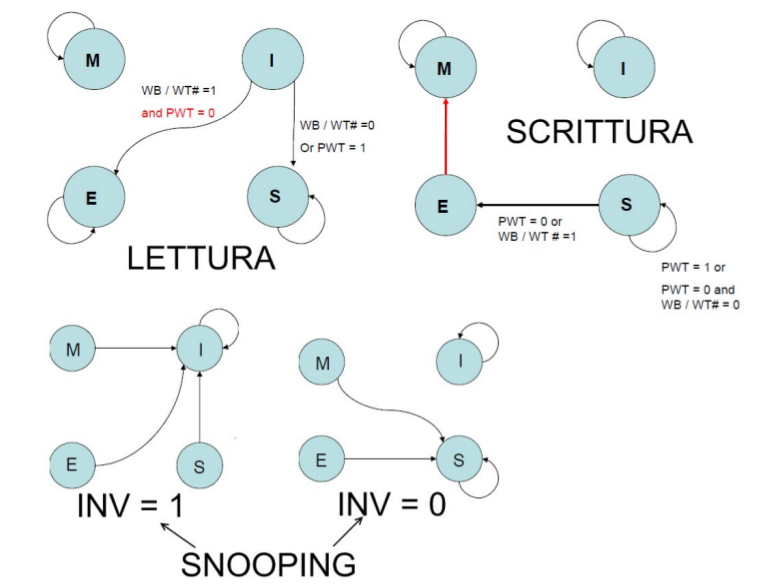
\includegraphics[width=\textwidth]{images/mesi.png}
  \caption{Stato MESI}
  \label{mesi}
\end{figure}

\appendix
\chapter{Le memorie associative}
\label{chap:memorieassociative}

Le {\bf memorie associative} sono memorie a cui si accede per
contenuto anzich\'e per indirizzo. Si differenziano dunque dalle RAM e
prendono il nome di {\bf CAM} ({\em Content Access Memory}). Le CAM
sono un componente fondamentale di tutte le moderne CPU e si
utilizzano in quasi ogni stadio della pipeline. Nello stadio IF ce ne
sono almeno 3, nello stadio EX ce n'\`e una per ogni unit\`a
funzionale, nello stadio MEM ce ne sono 2. Servono a velocizzare i
processi di traduzione degli indirizzi.  Per capire la differenza con
le RAM consideriamo che nelle RAM noi accediamo all'elemento che ha un
determinato indirizzo, nelle CAM invece accediamo al campo che ha un
determinato nome, indipendentemente da dove sia posizionato

\par\bigskip

Quando devo tradurre un indirizzo virtuale in fisico, un indirizzo di
memoria fisica in uno di cache o quando devo fare un predizione nel
caso di istruzioni di salto, allora ricorro alle CAM (la predizione
consiste nel calcolare il nuovo valore del PC da sostituire al
vecchio). 

\par\bigskip

Vediamo dunque alcune delle CAM che abbiamo nel calcolatore. La CAM
che traduce indirizzi virtuali in indirizzi fisici si chiama {\bf
  TLB}, cio\`e {\em Translation Look-Aside Buffer}. Abbiamo anche la
CAM che accelera la traduzione da PC vecchio a PC nuovo: questa si
chiama {\bf BTB}, {\em Branch Target Buffer}. Visto che le istruzioni
di salto (e quindi le traduzioni del PC) sono frequenti, conviene
avere delle BTB grandi. Anche le {\bf reservation station} sono delle
CAM, delle memorie associative su cui si scrive continuamente ci\`o
che arriva dal CRB (su cui viaggiano coppie nome-valore). La pi\`u
importante CAM \`e comunque la {\bf memoria cache}.

\par\bigskip

Le tabelle CAM oltre ad avere i campi {\bf nome} e {\bf valore}, hanno
un bit di validit\`a {\bf V/\={I}}. All'inizio ovviamente tutti i
campi saranno non validi (perci\`o avranno il bit posto a 0), poi man
mano che la CAM si riempe si pone a 1 tale bit. In realt\`a potremmo
avere un campo composto da pi\`u di un bit, nel caso in cui volessimo
specificare pi\`u informazioni, ma non lo vediamo per il momento.

\par\bigskip

Le memorie CAM possono essere organizzati in tre modi che ora
vedremo. Negli esempi vedremo come CAM la {\bf memoria cache}. In
questa CAM si entra con l'indirizzo fisico e, se c'\`e, si esce con la
relativa {\bf linea di cache}.

\section{Organizzazione Fully-Associative}

Le CAM {\bf Fully-Associative} sono quelle che hanno un comparatore
per ogni elemento della tabella.

\begin{figure}[h]
  \centering
  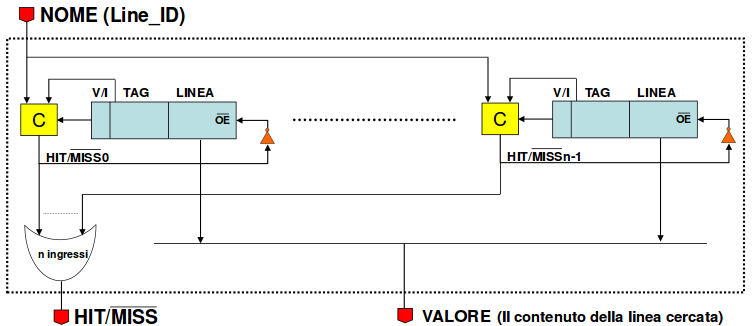
\includegraphics[width=.8\textwidth]{images/fullyassociative.png}
  \caption{Cache Fully-Associative}
  \label{fullyassociative}
\end{figure}

Nella figura, ogni tripla V/I - NOME - VALORE \`e rappresentata in
orizzontale. Quest'immagine si riferisce alla CAM che implementa la
cache, quindi il campo nome in realt\`a \`e l'{\bf indirizzo fisico},
il campo valore contiene invece la {\bf linea di cache}. 

\par\bigskip

Non si entra con tutto l'indirizzo fisico, ma solo con la parte che
identifica la linea di cache che si sta cercando. Ogni elemento della
CAM ha un comparatore in cui entrano l'identificatore della linea
cercata, il bit di validit\`a ed il campo nome di quella riga della
tabella. Tutti i comparatori effettuano il controllo e mandano l'esito
all'unica porta OR che determina cos\`i se c'\`e stato un {\bf HIT} o
un {\bf MISS}.

\par\bigskip

Sappiamo che la minima quantit\`a indirizzabile \`e il byte e che
abbiamo 32 bit di indirizzamento: vuol dire che riusciamo a mappare
$2^{32} = 4.294.967.296$ aree da 1 byte (diciamo che lo spazio di
indirizzamento \`e di 4 GB). Sapendo che le linee di cache sono da 32
byte (e 32 equivale a $2^5$) possiamo calcolare quante potenziali
linee ospita la memoria fisica: $2^{32} / 2^5 = 2^{27}$. Sono quindi
27 i bit che usiamo per identificare la linea e perci\`o come ingresso
della CAM. I 27 bit prendono il nome di {\bf LINE\_ID}. All'interno
della linea di cache si identifica il byte cercato con l'{\bf offset}
che \`e di 5 bit. La linea in uscita occupa 32 byte (cio\`e 256 bit,
dato che $32 byte = 2^3 \cdot 2^5 = 256 bit$). Quindi abbiamo dei
latch di 32 byte per memorizzare le linee. Solo uno di questi latch
contiene la linea che stiamo cercando (quindi solo un comparatore
pu\`s dare 1) e questo latch deve essere abilitato dal segnale di HIT
al trasferimento della linea sul bus, altrimenti rimane tristate.

\par\bigskip

Nelle CAM fully associative ogni nuovo elemento pu\`o essere inserito
in qualsiasi posizione della tabella. Al momento della ricerca di un
dato si va in parallelo ad analizzare ogni riga, pertanto i tempi son
brevissimi. Il tempo necessario per determinare se si ha un HIT o una
MISS \`e pari alla somma del tempo impiegato dai comparatori pi\`u il
tempo impiegato dall'OR. Il tempo necessario a mandare in output il
valore \`e pari alla somma del tempo impiegato dai comparatori pi\`u
il tempo dell'inverter che abilita la tristate pi\`u il tempo del
segnale OE che abilita la linea di cache. La cache fully associative
\`e dunque velocissima e garantisce un {\bf tempo di accesso costante}
per ogni locazione per\`o ha un {\bf costo elevato} che \`e dato dal
dover utilizzare un gran numero di comparatori. Ogni comparatore
individua una sola locazione, pertanto dovremo avere $n$ comparatori
per poter verificare tutte le locazioni della tabella. Abbiamo quindi
1 set ed $n$ vie. Il numero di vie \`e pari al numero di comparatori,
mentre il numero di set \`e dato dal numero di partizioni degli
indirizzi: nelle fully associative in ogni locazioni pu\`o andare ogni
indirizzo, quindi non si partiziona.

\section{Organizzazione a Mapping diretto}

Nel caso del mapping diretto abbiamo un unico comparatore, quindi
un'unica via. Ogni locazione della memoria fisica pu\`o andare solo in
una specifica cella della CAM. Alla stessa cella della CAM possono
essere destinate pi\`u locazioni della memoria fisica. Abbiamo quindi
che lo spazio degli indirizzi \`e partizionato in $n$ set a seconda di
dove possono andare le varie righe dello spazio di indirizzamento
fisico.  

\begin{figure}[h]
  \centering
  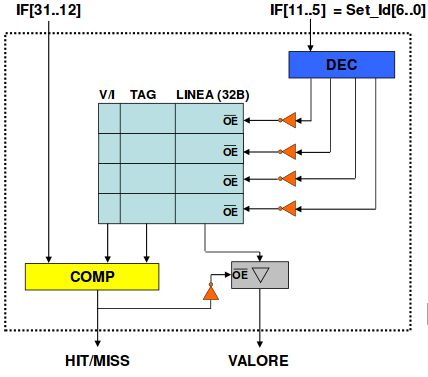
\includegraphics[width=.4\textwidth]{images/mappingdiretto.png}
  \caption{La cache a mapping diretto}
  \label{mappingdiretto}
\end{figure}

In questo caso abbiamo rappresentato le linee una sopra l'altra. Il
comparatore da solo non basta, serve anche un {\bf
  decoder}. L'indirizzo fisico si divide in due parti, una (la pi\`u
significativa) \`e il {\bf TAG} e l'altra \`e il {\bf SET\_ID}. Queste
insieme compongono quello che abbiamo chiamato {\bf LINE\_ID} nel
fully associative.

\par\bigskip

L'{\bf offset} (o Line Index) identifica il byte di interesse
all'interno della linea di cache selezionata; in questo esempio in cui
le linee di cache sono di 32 byte \`e di 5 bit. Il LINE\_ID \`e dato
ancora da $32-5=27$ bit. La dimensione del campo SET\_ID dipende dalla
dimensione della cache. Ad esempio una CAM di 128 linee richiede 7 bit
di SET\_ID. Questo vuol dire che dai 27 bit residui dovremmo togliere
i 7 bit per il SET\_ID e ce ne restano 20 che formano il TAG.

\par\bigskip

A seconda dei bit del SET\_ID, ogni locazione della memoria fisica
potr\`a andare solo nella relativa riga della CAM. Per semplicit\`a
consideriamo una CAM di 4 locazioni, perci\`o che richieda 2 bit. Ad
esempio una locazione di memoria fisica che ha i bit 00 nella
posizione del SET\_ID, pu\`o andare solo nella riga 00 della CAM. Di
indirizzi fisici che hanno 00 come SET\_ID ce n'\`e una moltitudine,
quindi nel momento in cui si va a recuperare una linea di cache per un
dato indirizzo fisico, non basta vedere qual \`e il SET\_ID e leggere
la relativa riga, bisogna anche confrontare i bit pi\`u significativi
con il campo TAG, per vedere che nella CAM ci sia effettivamente la
riga da noi cercata (il che darebbe un HIT). Una volta recuperata la
linea di cache di interesse (se presente) si legge il byte desiderato
utilizzando l'offset.

\par\bigskip

Ora vediamo cosa comporta il mapping diretto dal punto di vista delle
Miss. Innanzitutto diciamo che inizialmente le cache sono vuote quindi
al primo accesso ad ogni posizione della cache vi saranno
obbligatoriamente delle MISS che si chiamano appunto {\bf Miss
  obbligatorie} (o {\bf Miss Compulsory}). Supponiamo di voler
accedere in sequenza alle pagine 8,4,2,8. In memoria associativa
organizzata secondo Fully Associative, non appena si vede che il dato
non \`e presente in cache lo si inserisce in una posizione
qualunque. L'assenza del dato, considerando una cache inizialmente
vuota, ha generato la cosiddetta {\bf Miss Compulsory}. Nel caso del
mapping diretto ogni cella della memoria fisica pu\`o andare solo in
una ben determinata posizione della CAM. In particolare 8, 4 e 2 vanno
tutte nella cella 00 e questo genera dei miss diversi: la prima
richiesta della locazione 8 della memoria fisica fallisce trovando la
tabella vuota e ci\`o genera un Miss Compulsory, ma le successive
richieste delle pagine 4 e 2 e nuovamente 8 falliscono in quanto
trovano non lo spazio vuoto, ma la posizione gi\`a occupata da
un'altra cella. Questo si chiama {\bf Miss di conflitto} (la Miss di
conflitto pu\`o verificarsi solo nel mapping diretto). Esiste un altro
tipo di Miss ed \`e la miss di capacit\`a. Quando un programma ha una
{\bf footprint} (occupazione in memoria) di $n$ byte e la cache ha
dimensione pi\`u piccola, pu\`o capitare che il programma debba
sovrascrivere un'area della cache perch\'e ha gi\`a esaurito tutte le
locazioni che aveva a disposizione. Questa si chiama {\bf Miss di
  capacit\`a}. Questo tipo di Miss ci pu\`o essere sia nel Fully
Associative, sia nel mapping diretto. 

Nella fully associative la percentuale di Miss \`e migliore, ma il
costo \`e pi\`u elevato a causa del maggior numero di comparatori e
della maggior grandezza del campo TAG. Per questo si ricorre alla
soluzione intermedia, le cache set-associative.

\section{Organizzazione Set-Associative}

In questa struttura la cache, che consideriamo sempre di 128 byte,
viene organizzata come segue: se prima avevamo otto linee di cache in
colonna, adesso dividiamo quest'area in due finestre da quattro
colonne dette vie. Il {\bf SET\_ID} diventa di 2 bit perch\'e deve
individuare una fra quattro possibili linee, dunque il bit pi\`u
significativo del vecchio SET\_ID entra a far parte del tag. Nel
momento in cui bisogna memorizzare una linea di cache in una struttura
vuota \`e totalmente indifferente scegliere in quale delle due vie
memorizzarla una volta calcolato il SET\_ID. Questo vuol dire che ogni
locazione di memoria fisica pu\`o andare in due possibili posizioni
della cache. Quando una delle due \`e occupata si sceglie la posizione
libera, mentre quando entrambe sono occupate si avr\`a una {\bf Miss
  di conflitto} e pertanto si sostituisce quella utilizzata meno di
recente calcolata tramite l'algoritmo LRU.

\par\bigskip

Visto che il SET\_ID \`e di due bit, il decoder avr\`a quattro uscite
che servono a selezionare le relative linee in cache. Abbiamo poi due
comparatori, uno per ogni via, che servono a confrontare il TAG
dell'indirizzo fisico con il campo NOME della linea di cache.

\par\bigskip

In generale si possono avere $k$ vie. Questo tipo di memoria \`e fully
associative per ogni set. Le memorie set associative sono una via di
mezzo fra le memorie a mapping diretto (in cui abbiamo un comparatore
e $k=1$) e quelle fully associative (in cui abbiamo un comparatore per
ogni linea e $k$ \`e uguale al numero di linee). Le memorie fully
associative si ottengono da quelle set associative iterando il numero
di divisioni che effettuiamo sulla tabella. Questo porta ad una
diminuizione del numero di bit che formano il SET\_ID fino a che non
diventa pari a 0. Dividendo sempre di pi\`u riduciamo anche il numero
di miss di conflitto fino ad arrivare al caso delle fully associative
in cui questo tipo di Miss non si verifica.

\section{Politiche}

Supponiamo di dover aggiornare il valore di una locazione di memoria
che chiamiamo A[0]. Se questa \`e presente in cache si pu\`o scegliere
se aggiornare solo versione in cache o anche quella in memoria. La
prima politica si chiama {\bf Write Back}, la seconda {\bf Write
  Through}. Nel Write Back, finch\'e la linea non viene sostituita, si
mantengono due copie distinte di A[0]: una \`e quella in memoria, e
l'altra \`e quella pi\`u aggiornata situata in cache. Bisogna tener
traccia di questa situazione e lo si fa estendendo il campo stato
della linea. Finora avevamo detto che poteva essere Valid o Invalid,
ora bisogna distinguere altri casi: se il dato \`e valido lo posso
gestire tramite WB o tramite WT. Se lo gestisco con WB ho due
possibilit\`a: il dato in cache \`e diverso da quello in memoria
centrale (dato {\bf dirty}, sporco) oppure i due dati sono uguali
(dato {\bf clean}, pulito). Se lo gestisco tramite WT non ci sono
alternative, \`e pulito per definizione.

\par\bigskip

Abbiamo perci\`o quattro possibili stati: 

\begin{itemize}
\item Valido - gestito con WT
\item Valido - gestito con WB - dirty
\item Valido - gestito con WB - clean
\item Invalido
\end{itemize}

Servono pertanto 2 bit per lo stato.

\par\bigskip

Cosa succede se invece il dato non \`e presente in cache? Possiamo
trovare la relativa linea di cache vuota (campo di validit\`a pari a
0) oppure gi\`a occupata (campo pari a 1). Nel primo caso si genera
una {\bf Miss compulsory}, si fa un accesso in lettura alla memoria
per portare il dato in cache e contestualmente aggiorniamo la linea
inserita in cache secondo una delle politiche di scrittura viste
prima. Nel secondo caso invece si genera una {\bf Miss di scrittura}
perch\'e il campo \`e valido, ma non contiene il dato che ci
interessa. Possiamo perci\`o decidere se aggiornare il solo dato in
memoria ({\bf Write Around}) oppure portare il dato in cache (accesso
in lettura alla memoria fisica) e poi aggiornamento una volta portato
il dato in cache ({\bf Write Allocate}).

\begin{figure}[h]
  \centering
  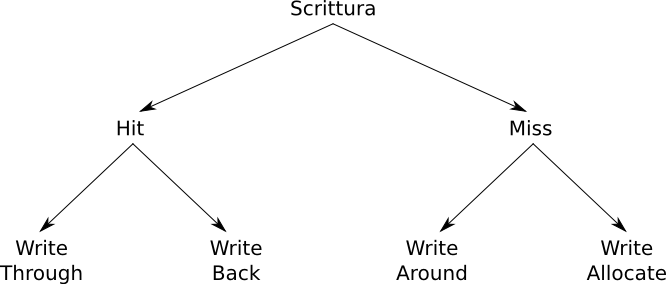
\includegraphics[width=.6\textwidth]{images/alberocache.png}
\end{figure}

La Write Through garantisce la coerenza della cache, ma richiede pi\`u
tempo.  Nel caso di Hit, la politica di scrittura adottata \`e una
caratteristica della linea di cache (cio\`e a seconda del valore
impostato nei bit di validit\`a si adotta una determinata politica),
mentre nel caso delle Miss la politica dipende dalla CPU. La Write
Allocate \`e molto complessa da implementare, pertanto molte delle CPU
moderne non la adottano.


\end{document}